\section*{Лекція 5: Умовні оператори}
 
 \subsection{Логічний тип даних} 
\begin{frame}
\frametitle{True та False}
\begin{itemize}
  \item True - істина
  \item False - брехня
 \end{itemize}

\begin{figure}
\begin{center}
 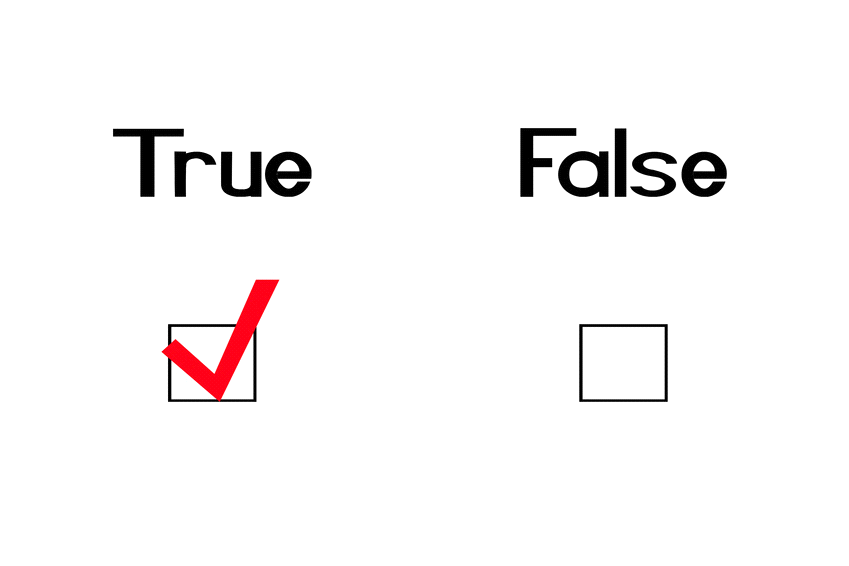
\includegraphics[width=0.4\textwidth]{pictures/TrueFalse.png}
\caption{True або False ?}
\label{TrueFalse} 
\end{center}
\end{figure}
\end{frame}

\begin{frame}
\frametitle{Логічні оператори}

\begin{table}
  \caption{Логічні вирази}
  \label{tab:}

  \begin{center}
    \begin{tabular}{|c|c|}
    \hline
      \textbf{Оператор} & \textbf{Значення} \\
    \hline  
      < & менше \\
    \hline
      >  & більше\\
    \hline
      <=  & менше або дорівнює \\
    \hline
      >=  & більше або дорівнює\\
    \hline
      ==  & дорівнює \\
    \hline
      !=  & не дорівнює \\
    \hline
    \end{tabular}
  \end{center}
\end{table}

\end{frame}

\begin{frame}
\frametitle{Логічні оператори}
\begin{table}
  \caption{Логічні оператори}
  \label{tab:}

  \begin{center}
    \begin{tabular}{|c|c|c|}
    \hline
      \textbf{Оператор} & \textbf{Значення} & \textbf{Пріоритет} \\
    \hline  
      or & або & 1 \\
    \hline
      and & та & 2 \\
    \hline
      not & ні & 3 \\
    \hline
    \end{tabular}
  \end{center}
\end{table}
\end{frame}

\subsection{Типове використання логічних операторів} 
\begin{frame}
\frametitle{Використання логічних операторів}
\begin{itemize}
  \item Перевірка на парність/непарність;
  \item Перевірка на потрапляння/непотрапляння в інтервал;
  \item Функція bool().
 \end{itemize}
\end{frame}

\subsection{Оператор розгалуження} 
\begin{frame}
\frametitle{Оператор if}
if - умовний оператор (оператор розгалуження).

% \begin{center}
\huge{if вираз:

~~~~операції}


\begin{flushleft}
\normalsize
Програма оцінює значення `вираз`, яке може дорівнювати True або False. Програма виконає операції тільки якщо вираз = True. Якщо вираз = False, цей шматок коду не буде виконуватись.
\end{flushleft}
% \end{center}
\end{frame}

\begin{frame}
\frametitle{Оператор if-else}
\Large{if вираз:

~~~~операції 1

else:

~~~~операції 2}


\begin{flushleft}
\normalsize
Операції 1 виконуються тільки якщо вираз істинний (дорівнює True). Якщо вираз дорівнює False, виконуються операції 2. Для розділення цих блоків використовуються відступи.
\end{flushleft}
% \end{center}
\end{frame}


\begin{frame}
\frametitle{Оператор if -elif-else}
\LARGE{if вираз 1:

~~~~операції 1

elif вираз 2:

~~~~операції 2

else:

~~~~операції 3}

\end{frame}

 \subsection{Використання умовного оператору} 
\begin{frame}
\frametitle{Знаходження мінімального}
\begin{figure}
\begin{center}
 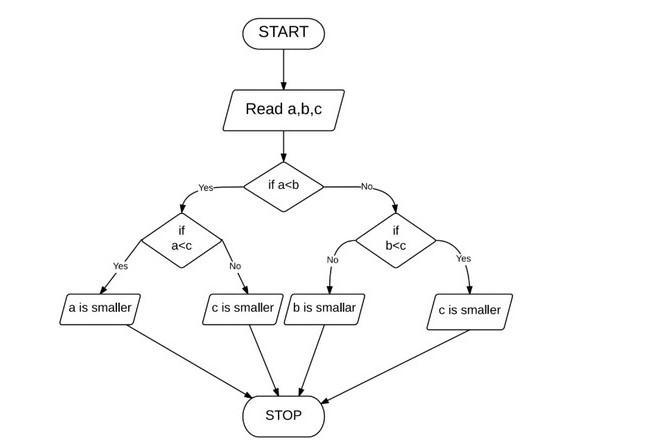
\includegraphics[width=0.4\textwidth]{pictures/find_min.jpg}
\caption{Алгоритм знаходження мінімального із трьох чисел}
\label{find_min} 
\end{center}
\end{figure}
\end{frame}

\begin{frame}
\frametitle{Тернарний умовний оператор}
У Python існує конструкція, яка за своєю дією аналогічна конструкції if-else, але є виразом. Вона називається тернарним оператором.

\Large{\texttt{значення\_1 if умова else значення\_2}}

Тернарний оператор повертає результат.
\end{frame}

\begin{frame}
\frametitle{Функції all та any}
Функція \texttt{all} повертає \texttt{True} якщо всі елементи переданого їй ітерованого об'єкту мають значення \texttt{True}.

Функція \texttt{any} повертає \texttt{True} якщо хоча б один елемент переданого їй ітерованого об'єкту має значення \texttt{True}.
\end{frame}

\subsection{Бітові операції} 
\begin{frame}
\frametitle{Операція НІ}
Бітова операція НІ виконує інверсію біт.

\begin{table}
  \caption{Бітова операція НІ}
  \label{tab:}

  \begin{center}
    \begin{tabular}{|c|c|}
    \hline
      \textbf{х} & \textbf{НІ} \\
    \hline
      0 & 1 \\
    \hline
      1 & 0 \\
    \hline
    \end{tabular}
  \end{center}
\end{table}

В Python бітова операція НІ позначається як $\sim x$.

\end{frame}

\begin{frame}
\frametitle{Операція І}

\begin{table}
  \caption{Бітова операція І: $x_1 \& x_2$}
  \label{tab:}

  \begin{center}
    \begin{tabular}{|c|c|c|}
    \hline
      \textbf{$x_1$} & \textbf{$x_2$} &  \textbf{І} \\
    \hline
      0 & 0 & 0 \\
    \hline
      0 & 1 & 0 \\
    \hline
      1 & 0 & 0 \\
    \hline
      1 & 1 & 1 \\
    \hline
    \end{tabular}
  \end{center}
\end{table}

Можна перевірити чи увімкнено або вимкнути відповідні біти.

\end{frame}

\begin{frame}
\frametitle{Операція АБО}

\begin{table}
  \caption{Бітова операція АБО: $x_1$ | $x_2$}
  \label{tab:}

  \begin{center}
    \begin{tabular}{|c|c|c|}
    \hline
      \textbf{$x_1$} & \textbf{$x_2$} &  \textbf{АБО} \\
    \hline
      0 & 0 & 0 \\
    \hline
      0 & 1 & 1 \\
    \hline
      1 & 0 & 1 \\
    \hline
      1 & 1 & 1 \\
    \hline
    \end{tabular}
  \end{center}
\end{table}

Можна перевірити чи увімкнено або вимкнути відповідні біти.

\end{frame}

\begin{frame}
\frametitle{Операція виключне АБО}

\begin{table}
  \caption{Бітова операція XOR: $x_1 \wedge x_2$}
  \label{tab:}

  \begin{center}
    \begin{tabular}{|c|c|c|}
    \hline
      \textbf{$x_1$} & \textbf{$x_2$} &  \textbf{XOR} \\
    \hline
      0 & 0 & 0 \\
    \hline
      0 & 1 & 1 \\
    \hline
      1 & 0 & 1 \\
    \hline
      1 & 1 & 0 \\
    \hline
    \end{tabular}
  \end{center}
\end{table}

За допомогою XOR можна перемикати біти числа.

\end{frame}

\begin{frame}
\frametitle{Зміщення біт}

\begin{itemize}
  \item $\gg$ - зміщення біт праворуч.
  \item  $\ll$  - зміщення біт ліворуч.

  \item $x = x \gg 1$ - еквівалентно цілочисленному діленню на два.

\end{itemize}


\end{frame}
